% This is the Reed College LaTeX thesis template. Most of the work
% for the document class was done by Sam Noble (SN), as well as this
% template. Later comments etc. by Ben Salzberg (BTS). Additional
% restructuring and APA support by Jess Youngberg (JY).
% Your comments and suggestions are more than welcome; please email
% them to cus@reed.edu
%
% See http://web.reed.edu/cis/help/latex.html for help. There are a
% great bunch of help pages there, with notes on
% getting started, bibtex, etc. Go there and read it if you're not
% already familiar with LaTeX.
%
% Any line that starts with a percent symbol is a comment.
% They won't show up in the document, and are useful for notes
% to yourself and explaining commands.
% Commenting also removes a line from the document;
% very handy for troubleshooting problems. -BTS

% As far as I know, this follows the requirements laid out in
% the 2002-2003 Senior Handbook. Ask a librarian to check the
% document before binding. -SN

%%
%% Preamble
%%
% \documentclass{<something>} must begin each LaTeX document
\documentclass[12pt,twoside]{reedthesis}
% Packages are extensions to the basic LaTeX functions. Whatever you
% want to typeset, there is probably a package out there for it.
% Chemistry (chemtex), screenplays, you name it.
% Check out CTAN to see: http://www.ctan.org/
%%
\usepackage{graphicx,latexsym}
\usepackage{amsmath}
\usepackage{amssymb,amsthm}
\usepackage{longtable,booktabs,setspace}
\usepackage{chemarr} %% Useful for one reaction arrow, useless if you're not a chem major
\usepackage[hyphens]{url}
% Added by CII
\usepackage{hyperref}
\usepackage{lmodern}
\usepackage{float}
\floatplacement{figure}{H}
% End of CII addition
\usepackage{rotating}

% Next line commented out by CII
%%% \usepackage{natbib}
% Comment out the natbib line above and uncomment the following two lines to use the new
% biblatex-chicago style, for Chicago A. Also make some changes at the end where the
% bibliography is included.
%\usepackage{biblatex-chicago}
%\bibliography{thesis}


% Added by CII (Thanks, Hadley!)
% Use ref for internal links
\renewcommand{\hyperref}[2][???]{\autoref{#1}}
\def\chapterautorefname{Chapter}
\def\sectionautorefname{Section}
\def\subsectionautorefname{Subsection}
% End of CII addition

% Added by CII
\usepackage{caption}
\captionsetup{width=5in}
% End of CII addition

% \usepackage{times} % other fonts are available like times, bookman, charter, palatino

% Syntax highlighting #22
  \usepackage{color}
  \usepackage{fancyvrb}
  \newcommand{\VerbBar}{|}
  \newcommand{\VERB}{\Verb[commandchars=\\\{\}]}
  \DefineVerbatimEnvironment{Highlighting}{Verbatim}{commandchars=\\\{\}}
  % Add ',fontsize=\small' for more characters per line
  \usepackage{framed}
  \definecolor{shadecolor}{RGB}{248,248,248}
  \newenvironment{Shaded}{\begin{snugshade}}{\end{snugshade}}
  \newcommand{\AlertTok}[1]{\textcolor[rgb]{0.94,0.16,0.16}{#1}}
  \newcommand{\AnnotationTok}[1]{\textcolor[rgb]{0.56,0.35,0.01}{\textbf{\textit{#1}}}}
  \newcommand{\AttributeTok}[1]{\textcolor[rgb]{0.77,0.63,0.00}{#1}}
  \newcommand{\BaseNTok}[1]{\textcolor[rgb]{0.00,0.00,0.81}{#1}}
  \newcommand{\BuiltInTok}[1]{#1}
  \newcommand{\CharTok}[1]{\textcolor[rgb]{0.31,0.60,0.02}{#1}}
  \newcommand{\CommentTok}[1]{\textcolor[rgb]{0.56,0.35,0.01}{\textit{#1}}}
  \newcommand{\CommentVarTok}[1]{\textcolor[rgb]{0.56,0.35,0.01}{\textbf{\textit{#1}}}}
  \newcommand{\ConstantTok}[1]{\textcolor[rgb]{0.00,0.00,0.00}{#1}}
  \newcommand{\ControlFlowTok}[1]{\textcolor[rgb]{0.13,0.29,0.53}{\textbf{#1}}}
  \newcommand{\DataTypeTok}[1]{\textcolor[rgb]{0.13,0.29,0.53}{#1}}
  \newcommand{\DecValTok}[1]{\textcolor[rgb]{0.00,0.00,0.81}{#1}}
  \newcommand{\DocumentationTok}[1]{\textcolor[rgb]{0.56,0.35,0.01}{\textbf{\textit{#1}}}}
  \newcommand{\ErrorTok}[1]{\textcolor[rgb]{0.64,0.00,0.00}{\textbf{#1}}}
  \newcommand{\ExtensionTok}[1]{#1}
  \newcommand{\FloatTok}[1]{\textcolor[rgb]{0.00,0.00,0.81}{#1}}
  \newcommand{\FunctionTok}[1]{\textcolor[rgb]{0.00,0.00,0.00}{#1}}
  \newcommand{\ImportTok}[1]{#1}
  \newcommand{\InformationTok}[1]{\textcolor[rgb]{0.56,0.35,0.01}{\textbf{\textit{#1}}}}
  \newcommand{\KeywordTok}[1]{\textcolor[rgb]{0.13,0.29,0.53}{\textbf{#1}}}
  \newcommand{\NormalTok}[1]{#1}
  \newcommand{\OperatorTok}[1]{\textcolor[rgb]{0.81,0.36,0.00}{\textbf{#1}}}
  \newcommand{\OtherTok}[1]{\textcolor[rgb]{0.56,0.35,0.01}{#1}}
  \newcommand{\PreprocessorTok}[1]{\textcolor[rgb]{0.56,0.35,0.01}{\textit{#1}}}
  \newcommand{\RegionMarkerTok}[1]{#1}
  \newcommand{\SpecialCharTok}[1]{\textcolor[rgb]{0.00,0.00,0.00}{#1}}
  \newcommand{\SpecialStringTok}[1]{\textcolor[rgb]{0.31,0.60,0.02}{#1}}
  \newcommand{\StringTok}[1]{\textcolor[rgb]{0.31,0.60,0.02}{#1}}
  \newcommand{\VariableTok}[1]{\textcolor[rgb]{0.00,0.00,0.00}{#1}}
  \newcommand{\VerbatimStringTok}[1]{\textcolor[rgb]{0.31,0.60,0.02}{#1}}
  \newcommand{\WarningTok}[1]{\textcolor[rgb]{0.56,0.35,0.01}{\textbf{\textit{#1}}}}

% To pass between YAML and LaTeX the dollar signs are added by CII
\title{Spatio temporal analysis of extreme wind velocities for infrastructure desing. Case study Colombia}
\author{Alexys Herleym Rodríguez Avellaneda}
% The month and year that you submit your FINAL draft TO THE LIBRARY (May or December)
\date{Jan 2020}
\division{Instituto for Geoinformatics - IFGI}
\advisor{Dr.~Edzer Pebesma}
\institution{University of Münster}
\degree{Master of Science in Geospatial Technologies}
%If you have two advisors for some reason, you can use the following
% Uncommented out by CII
\altadvisor{Dr.~Juan C. Reyes}
% End of CII addition

%%% Remember to use the correct department!
\department{}
% if you're writing a thesis in an interdisciplinary major,
% uncomment the line below and change the text as appropriate.
% check the Senior Handbook if unsure.
%\thedivisionof{The Established Interdisciplinary Committee for}
% if you want the approval page to say "Approved for the Committee",
% uncomment the next line
%\approvedforthe{Committee}

% Added by CII
%%% Copied from knitr
%% maxwidth is the original width if it's less than linewidth
%% otherwise use linewidth (to make sure the graphics do not exceed the margin)
\makeatletter
\def\maxwidth{ %
  \ifdim\Gin@nat@width>\linewidth
    \linewidth
  \else
    \Gin@nat@width
  \fi
}
\makeatother

\renewcommand{\contentsname}{Table of Contents}
% End of CII addition

\setlength{\parskip}{0pt}

% Added by CII

\providecommand{\tightlist}{%
  \setlength{\itemsep}{0pt}\setlength{\parskip}{0pt}}

\Acknowledgements{
I want to thank a few people.
}

\Dedication{
You can have a dedication here if you wish.
}

\Preface{
This is an example of a thesis setup to use the reed thesis document class
(for LaTeX) and the R bookdown package, in general.
}

\Abstract{
The preface pretty much says it all.

\par

Second paragraph of abstract starts here.
}

	\usepackage{booktabs}
\usepackage{longtable}
\usepackage{array}
\usepackage{multirow}
\usepackage{wrapfig}
\usepackage{float}
\usepackage{colortbl}
\usepackage{pdflscape}
\usepackage{tabu}
\usepackage{threeparttable}
\usepackage{threeparttablex}
\usepackage[normalem]{ulem}
\usepackage{makecell}
\usepackage{xcolor}
% End of CII addition
%%
%% End Preamble
%%
%
\begin{document}

% Everything below added by CII
  \maketitle

\frontmatter % this stuff will be roman-numbered
\pagestyle{empty} % this removes page numbers from the frontmatter
  \begin{acknowledgements}
    I want to thank a few people.
  \end{acknowledgements}
  \begin{preface}
    This is an example of a thesis setup to use the reed thesis document class
    (for LaTeX) and the R bookdown package, in general.
  \end{preface}
  \hypersetup{linkcolor=black}
  \setcounter{tocdepth}{2}
  \tableofcontents

  \listoftables

  \listoffigures
  \begin{abstract}
    The preface pretty much says it all.
    
    \par
    
    Second paragraph of abstract starts here.
  \end{abstract}
  \begin{dedication}
    You can have a dedication here if you wish.
  \end{dedication}
\mainmatter % here the regular arabic numbering starts
\pagestyle{fancyplain} % turns page numbering back on

\hypertarget{introduction}{%
\chapter*{Introduction}\label{introduction}}
\addcontentsline{toc}{chapter}{Introduction}

Placeholder
\begin{Shaded}
\begin{Highlighting}[]
\KeywordTok{library}\NormalTok{(knitr)}
\NormalTok{hook_output =}\StringTok{ }\NormalTok{knit_hooks}\OperatorTok{$}\KeywordTok{get}\NormalTok{(}\StringTok{'output'}\NormalTok{)}
\NormalTok{knit_hooks}\OperatorTok{$}\KeywordTok{set}\NormalTok{(}\DataTypeTok{output =} \ControlFlowTok{function}\NormalTok{(x, options) \{}
  \CommentTok{# this hook is used only when the linewidth option is not NULL}
  \ControlFlowTok{if}\NormalTok{ (}\OperatorTok{!}\KeywordTok{is.null}\NormalTok{(n <-}\StringTok{ }\NormalTok{options}\OperatorTok{$}\NormalTok{linewidth)) \{}
\NormalTok{    x =}\StringTok{ }\NormalTok{knitr}\OperatorTok{:::}\KeywordTok{split_lines}\NormalTok{(x)}
    \CommentTok{# any lines wider than n should be wrapped}
    \ControlFlowTok{if}\NormalTok{ (}\KeywordTok{any}\NormalTok{(}\KeywordTok{nchar}\NormalTok{(x) }\OperatorTok{>}\StringTok{ }\NormalTok{n)) x =}\StringTok{ }\KeywordTok{strwrap}\NormalTok{(x, }\DataTypeTok{width =}\NormalTok{ n)}
\NormalTok{    x =}\StringTok{ }\KeywordTok{paste}\NormalTok{(x, }\DataTypeTok{collapse =} \StringTok{'}\CharTok{\textbackslash{}n}\StringTok{'}\NormalTok{)}
\NormalTok{  \}}
  \KeywordTok{hook_output}\NormalTok{(x, options)}
\NormalTok{\})}
\end{Highlighting}
\end{Shaded}
\begin{Shaded}
\begin{Highlighting}[]
\CommentTok{# List of packages required for this analysis}
\NormalTok{pkg <-}\StringTok{ }\KeywordTok{c}\NormalTok{(}\StringTok{"dplyr"}\NormalTok{, }\StringTok{"sf"}\NormalTok{, }\StringTok{"ggplot2"}\NormalTok{,}\StringTok{"rnaturalearth"}\NormalTok{, }\StringTok{"rnaturalearthdata"}\NormalTok{, }
         \StringTok{"ggspatial"}\NormalTok{, }\StringTok{"kableExtra"}\NormalTok{, }\StringTok{"ncdf4"}\NormalTok{, }\StringTok{"stars"}\NormalTok{, }\StringTok{"magick"}\NormalTok{, }\StringTok{"RcmdrMisc"}\NormalTok{,}
         \StringTok{"knitr"}\NormalTok{, }\StringTok{"bookdown"}\NormalTok{, }\StringTok{"devtools"}\NormalTok{)}
\CommentTok{# Check if packages are not installed and assign the}
\CommentTok{# names of the packages not installed to the variable new.pkg}
\NormalTok{new.pkg <-}\StringTok{ }\NormalTok{pkg[}\OperatorTok{!}\NormalTok{(pkg }\OperatorTok\StringTok{ }\KeywordTok{installed.packages}\NormalTok{())]}
\CommentTok{# If there are any packages in the list that aren't installed,}
\CommentTok{# install them}
\ControlFlowTok{if}\NormalTok{ (}\KeywordTok{length}\NormalTok{(new.pkg))}
  \KeywordTok{install.packages}\NormalTok{(new.pkg, }\DataTypeTok{repos =} \StringTok{"http://cran.rstudio.com"}\NormalTok{)}
\CommentTok{# Load packages (thesisdown will load all of the packages as well)}
\KeywordTok{library}\NormalTok{(}\StringTok{"thesisdown"}\NormalTok{)}
\KeywordTok{library}\NormalTok{(}\StringTok{"dplyr"}\NormalTok{)}
\KeywordTok{library}\NormalTok{(}\StringTok{"sf"}\NormalTok{)}
\KeywordTok{library}\NormalTok{(}\StringTok{"ggplot2"}\NormalTok{)}
\KeywordTok{library}\NormalTok{(}\StringTok{"rnaturalearth"}\NormalTok{)}
\KeywordTok{library}\NormalTok{(}\StringTok{"rnaturalearthdata"}\NormalTok{)}
\KeywordTok{library}\NormalTok{(}\StringTok{"ggspatial"}\NormalTok{)}
\CommentTok{#library("tibble")}
\KeywordTok{library}\NormalTok{(}\StringTok{"knitr"}\NormalTok{)}
\KeywordTok{library}\NormalTok{(}\StringTok{"kableExtra"}\NormalTok{)}
\KeywordTok{library}\NormalTok{(}\StringTok{"ncdf4"}\NormalTok{)}
\KeywordTok{library}\NormalTok{(}\StringTok{"stars"}\NormalTok{)}
\KeywordTok{library}\NormalTok{(}\StringTok{"magick"}\NormalTok{)}
\KeywordTok{library}\NormalTok{(}\StringTok{"RcmdrMisc"}\NormalTok{)}
\end{Highlighting}
\end{Shaded}
\hypertarget{rmd-data}{%
\chapter{Data}\label{rmd-data}}

Input data is made up of three different sources a) IDEAM - Institute of Hydrology, Meteorology and Environmental Studies of Colombia \url{http://www.ideam.gov.co}, b) ISD - Integrated Surface Database \url{https://www.ncdc.noaa.gov/isd}, and c) ERA5 climate reanalysis \url{https://www.ecmwf.int/en/forecasts/datasets/reanalysis-datasets/era5}.

\begingroup\fontsize{10}{12}\selectfont
\begin{longtable}[t]{l>{\raggedright\arraybackslash}p{0.8in}>{\raggedright\arraybackslash}p{4in}}
\caption[Datasets]{\label{tab:tabledatasources1}Datasets description}\\
\toprule
\multicolumn{1}{l}{Institution} & \multicolumn{1}{l}{Dataset} & \multicolumn{1}{l}{Details}\\
\midrule
IDEAM & Historical records at weather stations & IDEAM is responsible for the instalation, maintenance and management of all kind of weather stations located everywhere along the country\\
NOAA & ISD & ISD (Integrated Surface Database. NOAA's National Centers for Environmental Information - NCEI) Lite: A subset from the full ISD dataset containing eight common surface parameters in a fixed-width format free of duplicate values, sub-hourly data, and complicated flags.\\
ECMWF & ERA5 & ERA5 is a reanalysis dataset with hourly estimates of atmospheric variables with horizontal resolution of 0.25º (33 kilómeters), this is equally spaced cells every 0.25 degrees\\
\bottomrule
\end{longtable}
\endgroup{}

\begingroup\fontsize{10}{12}\selectfont
\begin{longtable}[t]{l>{\raggedright\arraybackslash}p{1.2in}>{\raggedright\arraybackslash}p{3.5in}}
\caption[Variables]{\label{tab:tabledatasources2}Datasets variables}\\
\toprule
\multicolumn{1}{l}{Dataset} & \multicolumn{1}{l}{Variables} & \multicolumn{1}{l}{Description}\\
\midrule
IDEAM & vvmx\_aut\_60 & Hourly wind maximun velocity\\
ISD & wind speed rate & Maximun hourly wind velocity. The rate of horizontal travel of air past a fixed point.\\
ERA5 & fg10 & 10 metre wind gust since previous post-processing\\
 & fsr & Forecast Surface Roughness\\
\bottomrule
\end{longtable}
\endgroup{}

\begingroup\fontsize{10}{12}\selectfont
\begin{longtable}[t]{l>{\raggedright\arraybackslash}p{0.8in}>{\raggedright\arraybackslash}p{3in}l}
\caption[Units and Time]{\label{tab:tabledatasources3}Variables units and time}\\
\toprule
\multicolumn{1}{l}{Variable} & \multicolumn{1}{l}{Units} & \multicolumn{1}{l}{Time} & \multicolumn{1}{l}{Stations}\\
\midrule
vvmx\_aut\_60 & meters per second & Variable from 2001 until today. Irregular time series. & 203\\
Wind speed & meters per second & Variable from 1941 until today. Note: There is too much variability in time (start, end, and time range) for each station. Irregutal time series. & 101\\
fg10 & meters per second & 1979-Today & 3381\\
fsr & meters per second & 1979-Today & 3381\\
\bottomrule
\end{longtable}
\endgroup{}

Ideal data source to create extreme wind speeds maps should be field observed data from IDEAM, but there are not enough number of stations around the study area to represent all the local wind variability in a huge country with multiple variety of climates and and changing thermal floors, but there are other important motivatios to include different sources trying to improve output results:
\begin{itemize}
\tightlist
\item
  As just mentioned, low quantity of IDEAM stations
\item
  There are uncertanties related to the way IDEAM anemometers are registering data, then comparison with other datasources are needed to be able to do appropriate data standardization, needed as a prerequisite to the analysis.
\item
  There is no time continuity in the registration of IDEAM data. Historical time series are different and variable in each station.
\end{itemize}
Importance of ISD database for this study is based on the fact that post-procesed ISD database has wind extreme values, and it was used to create extreme wind maps for United States. ISD allows comparison with IDEAM records to take better decitions in order to do needed data standarization.

Despite that ERA5 data are not observed data, but forecast, its main advantage is data availability to assess the local climatic variance every 33 square kilometers.

\hypertarget{ideam}{%
\section{IDEAM}\label{ideam}}

\textbf{R}
\begin{itemize}
\tightlist
\item
  Item 1
\item
  Item 2
\end{itemize}
\begin{enumerate}
\def\labelenumi{\arabic{enumi}.}
\item
  Item 1
\item
  Item 2
\item
  Item 1
\item
  Item 2
\item
  Item 3
  \begin{itemize}
  \tightlist
  \item
    Item 3a
  \item
    Item 3b
  \end{itemize}
\end{enumerate}
Historical observed wind speeds from 203 in Colombia are managed by the official environmental authority IDEAM. Table \ref{tab:tableideamstations} shows a sample of five IDEAM stations. Figure \ref{fig:plotideamstations} shows a map of IDEAM stations.
\begin{longtable}[t]{lrr}
\caption[IDEAM Stations]{\label{tab:tableideamstations}IDEAM Stations sample}\\
\toprule
Name[Code] & Latitud & Longitud\\
\midrule
EMAS - AUT [26155230] & 5.09 & -75.51\\
SAN BENITO - AUT [25025380] & 9.16 & -75.04\\
AEROPUERTO ALFONSO LOPEZ - [28025502] & 10.44 & -73.25\\
TIBAITATA - AUT [21206990] & 4.69 & -74.21\\
ELDORADO CATAM - AUT [21205791] & 4.71 & -74.15\\
\bottomrule
\end{longtable}
\begin{figure}
\centering
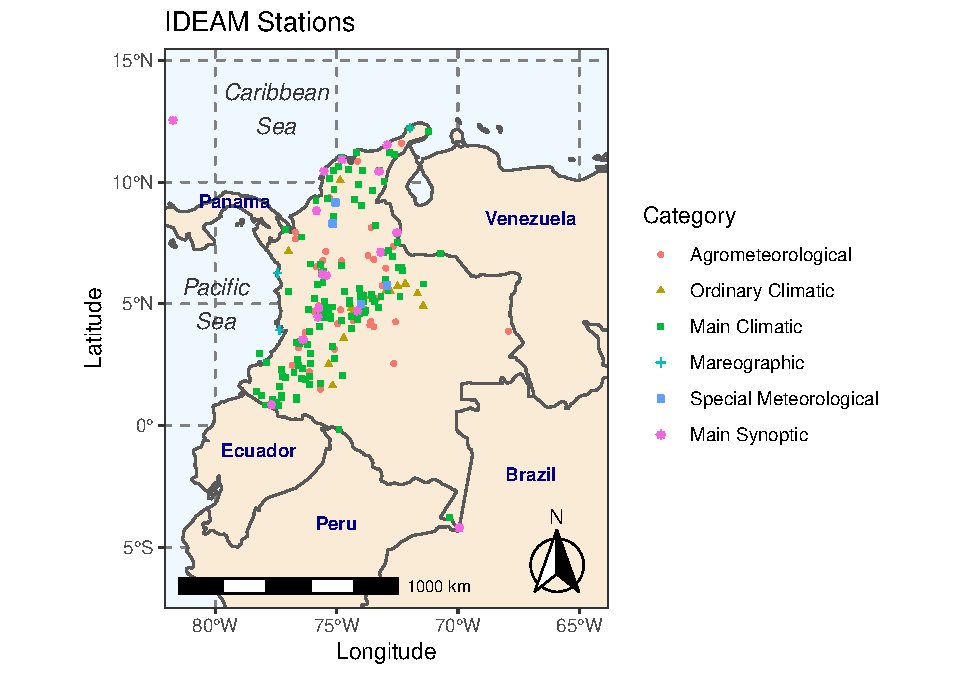
\includegraphics{thesis_files/figure-latex/plotideamstations-1.pdf}
\caption{\label{fig:plotideamstations}IDEAM Stations}
\end{figure}
Following, the time serie for the IDEAM station ``21205791'' will be displayed
\begin{verbatim}
select "mydatetime", "21205791" as "X21205791" from ideam_vvmx_60 where "21205791" IS NOT NULL
\end{verbatim}
\begin{figure}
\centering
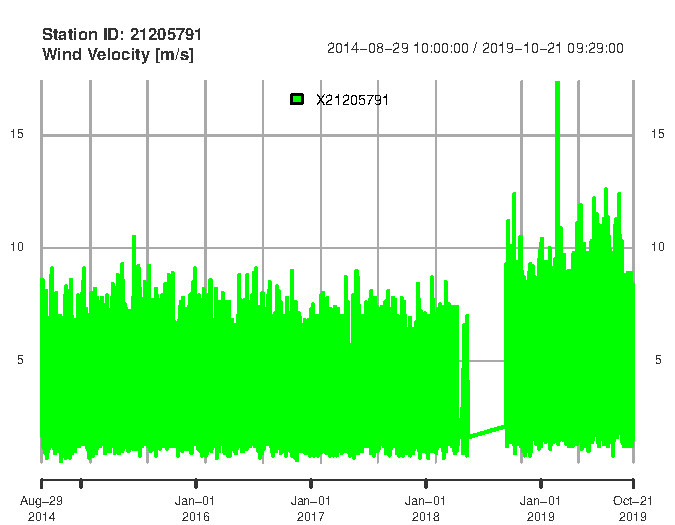
\includegraphics{thesis_files/figure-latex/plotoneideamstation-1.pdf}
\caption{\label{fig:plotoneideamstation}IDEAM Station}
\end{figure}
\begin{figure}
\centering
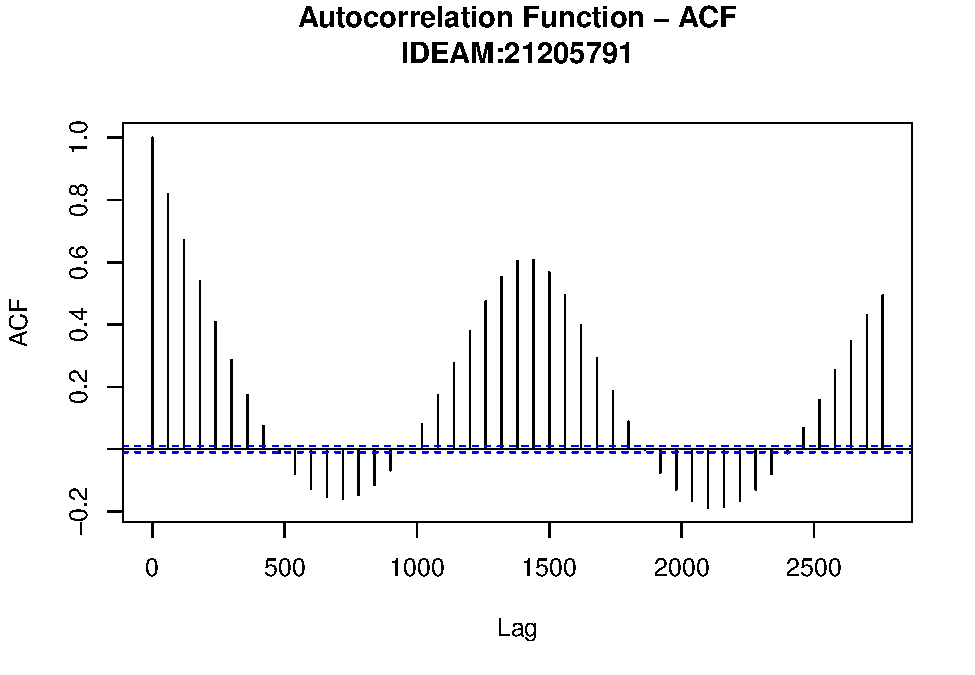
\includegraphics{thesis_files/figure-latex/plotoneideamstationacf-1.pdf}
\caption{\label{fig:plotoneideamstationacf}IDEAM Station}
\end{figure}
\begin{figure}
\centering
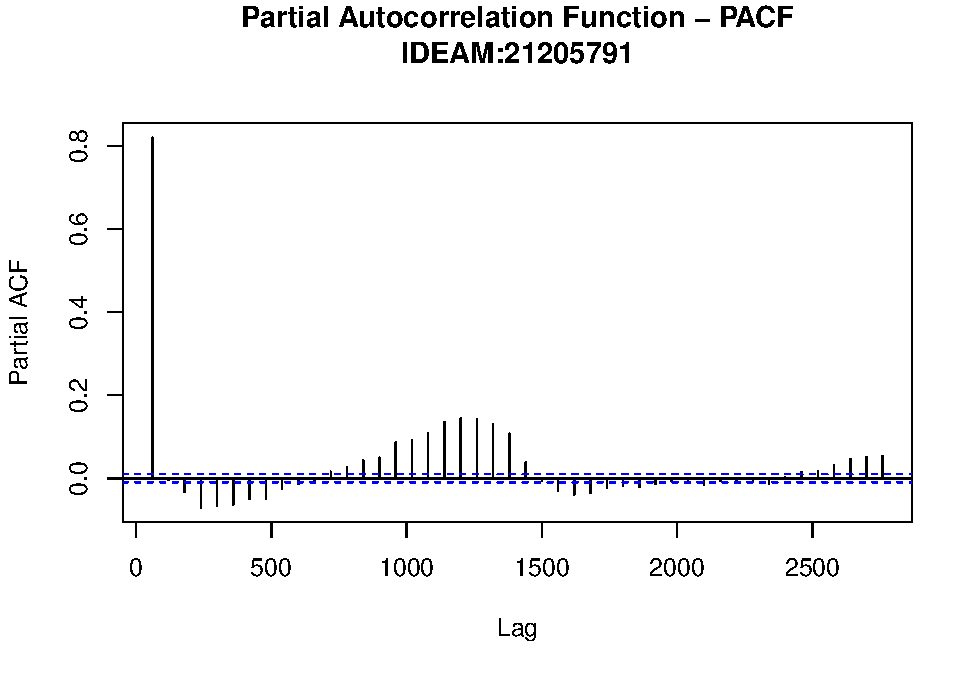
\includegraphics{thesis_files/figure-latex/plotoneideamstationpacf-1.pdf}
\caption{\label{fig:plotoneideamstationpacf}IDEAM Station}
\end{figure}
\hypertarget{isd}{%
\section{ISD}\label{isd}}

\emph{Now for the correct way:}
ISD is a database with environmental variables among then extreme wind speeds. ISD has data for the whole planet, and is based on observed data at metereological stations in each country, which means that for Colombia is based on IDEAM data. Main advantage is data availability at neighbor countries and specialized postprocesing made by NOAA's National Centers for Environmental Information - NCEI in United States, which facilitates its use.Table \ref{tab:tableisdstations} shows a sample of five ISD stations. Figure \ref{fig:plotisdstations} shows a map of ISD stations.
\begin{longtable}[t]{llrr}
\caption[ISD Stations]{\label{tab:tableisdstations}ISD Stations sample}\\
\toprule
Code & Name & Latitud & Longitud\\
\midrule
804400 & BARINAS & 8.62 & -70.22\\
800810 & ALTO CURICHE & 7.05 & -76.35\\
801000 & BAHIA SOLANO / JOSE MUTIS & 6.18 & -77.40\\
802590 & ALFONSO BONILLA ARAGON INTL & 3.54 & -76.38\\
803150 & BENITO SALAS & 2.95 & -75.29\\
\bottomrule
\end{longtable}
\begin{figure}
\centering
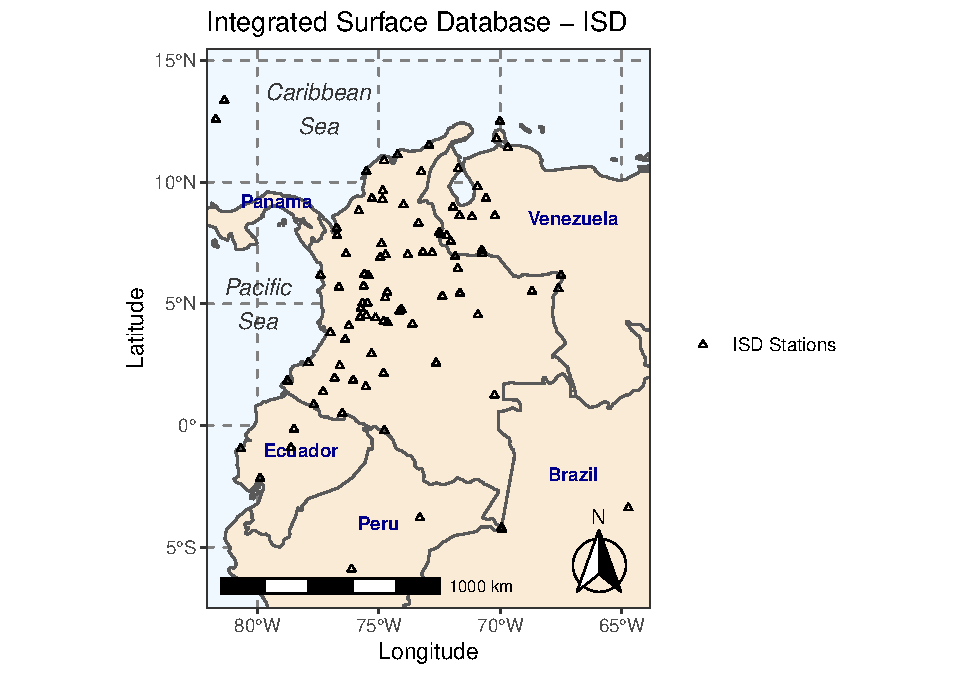
\includegraphics{thesis_files/figure-latex/plotisdstations-1.pdf}
\caption{\label{fig:plotisdstations}ISD Stations}
\end{figure}
\hypertarget{era5}{%
\section{ERA5}\label{era5}}

ERA5 is forecast reanalysis data procesed by the \emph{European Centre for Medium-Range Weather Forecasts} - ECMWF with wind speeds time series in square cells \emph{matrix of pixels} of 0.25 degrees (33 km) covering the whole plannet. For the study area was extracted a raster of 69 rows by 49 XXX columns in format NetCDF. Figure \ref{fig:plotera5stations} shows a map of ERA5 stations (cells centers).
\begin{figure}
\centering
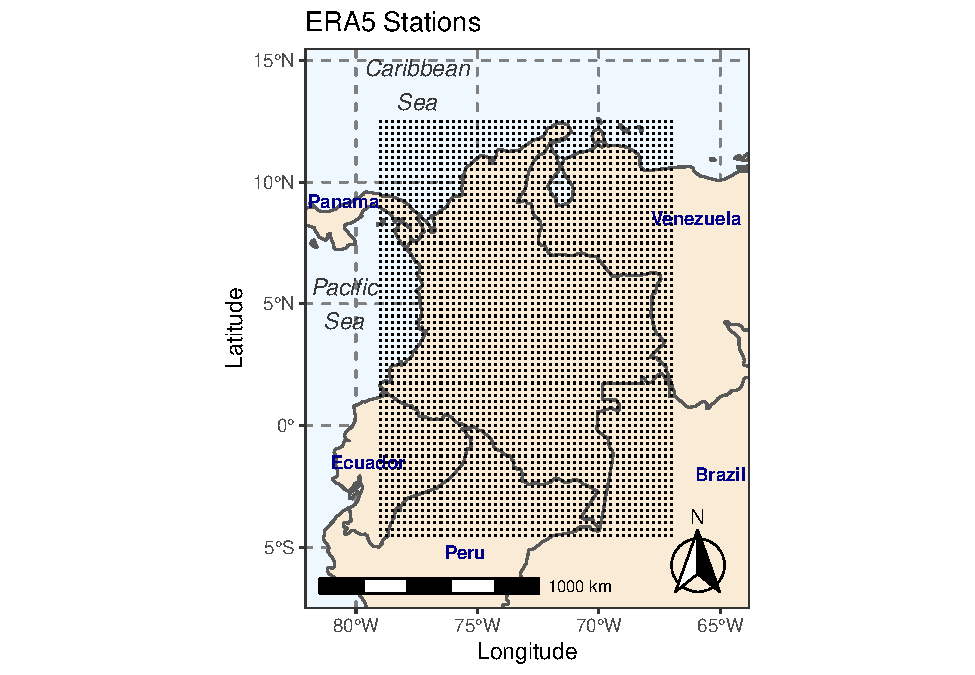
\includegraphics{thesis_files/figure-latex/plotera5stations-1.pdf}
\caption{\label{fig:plotera5stations}ERA5 Stations (cells centers)}
\end{figure}
\hypertarget{section}{%
\section{}\label{section}}

\hypertarget{data-download-and-organization}{%
\section{Data Download and Organization}\label{data-download-and-organization}}

\hypertarget{data-standarzation}{%
\section{Data Standarzation}\label{data-standarzation}}

Analysis of extreme wind speeds requieres data standarizaton as initial step. All input data must be standarized to represent three important conditions: a) anemometer height of 10 meters, b) open space roughness, and c) averaging time of 3-seconds wind gust. Data for analysis must represent 3-s peak wind speeds 10 meters heigh above the surface, in open terrain.
* 10 mts anemometer height
* Open space terrain roughness
* 3-s gust averaging time
\begin{quote}
The \texttt{cos} of \(2 \pi\) is 1.
\end{quote}
\begin{quote}
The standard deviation of \texttt{speed} in \texttt{cars} is 5.2876444.
\end{quote}
\begin{quote}
The standard deviation is less than 6.
\end{quote}
As you see with \texttt{\$2\ \textbackslash{}pi\$} above, mathematics can be added by surrounding the mathematical text with dollar signs. More examples of this are in {[}Mathematics and Science{]} if you uncomment the code in {[}Math{]}.

\textbf{\emph{after}} you have run the \textbf{R}

\clearpage

\hypertarget{rmd-thefra}{%
\chapter{Theoretical Framework}\label{rmd-thefra}}

Placeholder

\hypertarget{probability-concepts}{%
\section{Probability Concepts}\label{probability-concepts}}

\hypertarget{probability-density-function---pdf}{%
\subsection{\texorpdfstring{Probability Density Function - \emph{pdf}}{Probability Density Function - pdf}}\label{probability-density-function---pdf}}

\hypertarget{cumulative-distribution-funtcion---cdf}{%
\subsection{\texorpdfstring{Cumulative Distribution Funtcion - \emph{cdf}}{Cumulative Distribution Funtcion - cdf}}\label{cumulative-distribution-funtcion---cdf}}

\hypertarget{percent-point-function---ppf}{%
\subsection{\texorpdfstring{Percent Point Function - \emph{ppf}}{Percent Point Function - ppf}}\label{percent-point-function---ppf}}

\hypertarget{hazard-function---hf}{%
\subsection{\texorpdfstring{Hazard Function - \emph{hf}}{Hazard Function - hf}}\label{hazard-function---hf}}

\hypertarget{cumulative-hazard-function}{%
\subsection{Cumulative Hazard Function}\label{cumulative-hazard-function}}

\hypertarget{annual-excedance-probability---pa}{%
\section{Annual Excedance Probability - Pa}\label{annual-excedance-probability---pa}}

\hypertarget{typesetting-reactions}{%
\subsection{Typesetting reactions}\label{typesetting-reactions}}

\hypertarget{other-examples-of-reactions}{%
\subsection{Other examples of reactions}\label{other-examples-of-reactions}}

\hypertarget{return-period}{%
\section{Return Period}\label{return-period}}

\hypertarget{compound-excedance-probability---pn}{%
\section{Compound Excedance Probability - Pn}\label{compound-excedance-probability---pn}}

\hypertarget{extreme-value-analysis-overview}{%
\section{Extreme Value Analysis Overview}\label{extreme-value-analysis-overview}}

\hypertarget{main-methods}{%
\subsection{Main Methods}\label{main-methods}}

\hypertarget{epochal-methods}{%
\subsubsection{Epochal methods}\label{epochal-methods}}

\hypertarget{peak-over-threshold}{%
\subsubsection{Peak Over Threshold}\label{peak-over-threshold}}

\hypertarget{gpd}{%
\paragraph{GPD}\label{gpd}}

\hypertarget{poisson-process}{%
\paragraph{Poisson Process}\label{poisson-process}}

\hypertarget{commond-distributions-for-extreme-values}{%
\subsection{Commond Distributions for Extreme Values}\label{commond-distributions-for-extreme-values}}

\hypertarget{methods-for-parameters-estimation}{%
\subsection{Methods for parameters estimation}\label{methods-for-parameters-estimation}}

\hypertarget{return-period-1}{%
\subsection{Return Period}\label{return-period-1}}

\hypertarget{wind-speed-at-return-period}{%
\subsection{Wind Speed at Return Period}\label{wind-speed-at-return-period}}

\hypertarget{rmd-method}{%
\chapter{Methodology}\label{rmd-method}}

Placeholder

\hypertarget{input-data-selection-and-standarization}{%
\section{Input Data Selection and Standarization}\label{input-data-selection-and-standarization}}

\hypertarget{data-selection}{%
\subsection{Data Selection}\label{data-selection}}

\hypertarget{data-standarization}{%
\subsection{Data Standarization}\label{data-standarization}}

\hypertarget{anemometer-height---10-m}{%
\subsubsection{Anemometer height - 10 m}\label{anemometer-height---10-m}}

\hypertarget{surface-roughness---0.03-m}{%
\subsubsection{Surface Roughness - 0.03 m}\label{surface-roughness---0.03-m}}

\hypertarget{averaging-time---3-s-gust}{%
\subsubsection{Averaging Time - 3-s gust}\label{averaging-time---3-s-gust}}

\hypertarget{fit-data-to-a-pot---poisson-process}{%
\section{Fit data to a POT - Poisson Process}\label{fit-data-to-a-pot---poisson-process}}

\hypertarget{velocities-at-return-periods}{%
\subsection{Velocities at Return Periods}\label{velocities-at-return-periods}}

\hypertarget{spatial-interpolation}{%
\section{spatial Interpolation}\label{spatial-interpolation}}

\hypertarget{footnotes-and-endnotes}{%
\section{Footnotes and Endnotes}\label{footnotes-and-endnotes}}

\hypertarget{bibliographies}{%
\section{Bibliographies}\label{bibliographies}}

\hypertarget{anything-else}{%
\section{Anything else?}\label{anything-else}}

\hypertarget{conclusion}{%
\chapter*{Conclusion}\label{conclusion}}
\addcontentsline{toc}{chapter}{Conclusion}

If we don't want Conclusion to have a chapter number next to it, we can add the \texttt{\{-\}} attribute.

\textbf{More info}

And here's some other random info: the first paragraph after a chapter title or section head \emph{shouldn't be} indented, because indents are to tell the reader that you're starting a new paragraph. Since that's obvious after a chapter or section title, proper typesetting doesn't add an indent there.

\appendix

\hypertarget{the-first-appendix}{%
\chapter{The First Appendix}\label{the-first-appendix}}

This first appendix includes all of the R chunks of code that were hidden throughout the document (using the \texttt{include\ =\ FALSE} chunk tag) to help with readibility and/or setup.

\textbf{In the main Rmd file}

\textbf{In Chapter \ref{rmd-method}:}

\hypertarget{the-second-appendix-for-fun}{%
\chapter{The Second Appendix, for Fun}\label{the-second-appendix-for-fun}}

\hypertarget{references}{%
\chapter*{References}\label{references}}
\addcontentsline{toc}{chapter}{References}

Placeholder


% Index?

\end{document}
